% TODO:
%    - Proposal Generation 
%    - Feature representation learning
%    - Add seprate title for background cocepts "Deep learning": speak about deep neural network
%
%

\chapter{Détection d'objets et apprentissage profond}
\newpage
\pagestyle{fancy}
\fancyhead[L]{\chaptername \ \thechapter}
\fancyhead[R]{Détection d'objets et apprentissage profond}
\renewcommand{\headrulewidth}{1pt}
\fancyfoot[C]{\thepage}
\section{Introduction} 
Au début de l'intelligence artificielle avec la limitation des ressources de calcul, les chercheurs ou les programmeurs devaient choisir et extraire manuellement les caractéristiques, puis appliquer un algorithme tel que la régression ou la classification en fonction des caractéristiques extraites. Cela a limité les performances des modèles et ses résultats en raison des capacités limitées d'un humain à extraire les bonnes caractéristiques, en particulier lorsque les données contiennent une grande quantité de caractéristiques à extraire, ce qui affecte considérablement les performances des modèles.

Avec l'augmentation drastique de la puissance de calcul du matériel moderne, cela a permis d'implémenter un nouvel algorithme qui a résolu le problème précédent d'extraction de caractéristiques et a également créé un nouveau domaine d'intelligence artificielle qui est l'apprentissage en profondeur.

L'apprentissage en profondeur est basé sur des réseaux de neurones avec de nombreuses couches cachées qui, à leur tour, effectuent l'extraction de caractéristiques avec l'objectif du modèle (comme la classification). La première couche du réseau de neurones qui est la couche d'entrée (certains ne l'appellent pas une couche car elle ne contient aucun neurone). Cette couche transmet les données à la couche suivante où résident réellement des neurones, chaque neurone reçoit 1 ou plusieurs entrées de la couche précédente, puis applique un algorithme de calcul tel que : Régression linéaire \(Z = W * X + b\) où w est le poids ou Convolution : \(Z = X * f\) où les valeurs X du noyau sont les poids du neurone. Après avoir calculé Z, la valeur est transmise à une fonction d'activation spécifique telle que : \(ReLu(x) = max(0,x)\) puis la valeur finale est transmise en tant qu'entrée pour la couche suivante jusqu'à ce qu'elle atteigne la couche finale qui produit la prédiction du modèle. Ces étapes sont appelées propagation vers l'avant là où le modèle prédit. 

D'autre part, la rétroporpagation où le modèle apprend, il fait que l'erreur après avoir calculé en comparant les sorties souhaitées aux sorties du modèle prédites, puis en la propageant aux couches précédentes où, pour chaque neurone, les poids sont ajustés en fonction de l'algorithme d'optimisation choisi comme : Gradient Descent.
\begin{figure}[H]
     \centering
     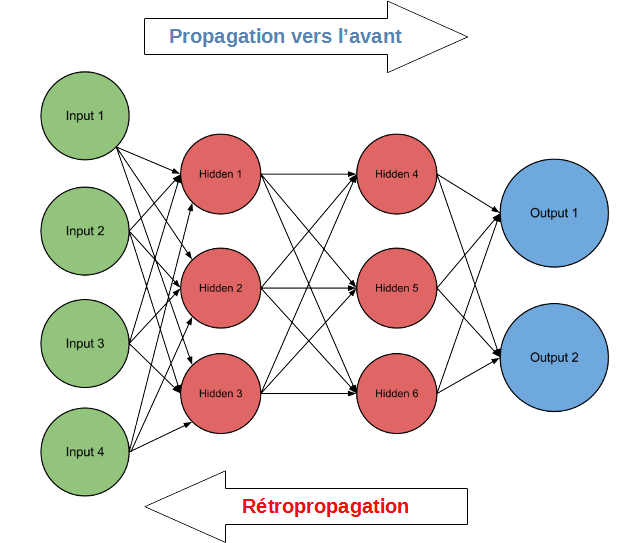
\includegraphics[height=12cm,width=12cm]{Chapitre2/img1.png}
     \caption{Structure d'un réseaux de neurones.}
     \label{img1}
     \end{figure}

\section{Concepts de base} 
% =========== CNN =========== 
     \subsection{Les réseaux de neurones convolutifs (CNN)} 
     De nombreux types de réseaux de neurones sont apparus pour résoudre des problèmes spécifiques, l'un d'eux est le réseau de neurones convolutifs (CNN), un réseau de neurones bien adapté pour traiter des tâches liées à la vision comme la reconnaissance d'objets. Ils ont été introduits pour la première fois en 1989, mais avec l'augmentation des pouvoirs de calcul et les grands ensembles de données d'imagerie, ils sont devenus le type de réseau neuronal de pointe pour la vision numérique.
     
     La structure CNN est inspirée du cortex visuel chez les animaux, où des groupes de cellules sont sensibles à une petite sous-région de l'image d'entrée. Par conséquent, l'image n'est pas traitée comme un bloc unique mais comme une composition d'éléments plus petits. \cite{db3}
     
     Le réseau de neurones contient plusieurs types de couches, chacune ayant un objectif spécifique et les couches les plus importantes sont :
     
     % =========== Convolution Layer =========== 
     \subsubsection{Couche de convolution}   
     La couche de convolution est la pierre angulaire du CNN. Il porte la partie principale de la charge de calcul du réseau où il effectue un produit scalaire entre 2 matrices : la première est le noyau, un ensemble de poids apprenables qui sont également les caractéristiques extraites et la seconde matrice est un ensemble de valeurs contenues dans le glissement fenêtre sur l'image, glissant d'un pas donné.
     \begin{figure}[H]
          \centering
          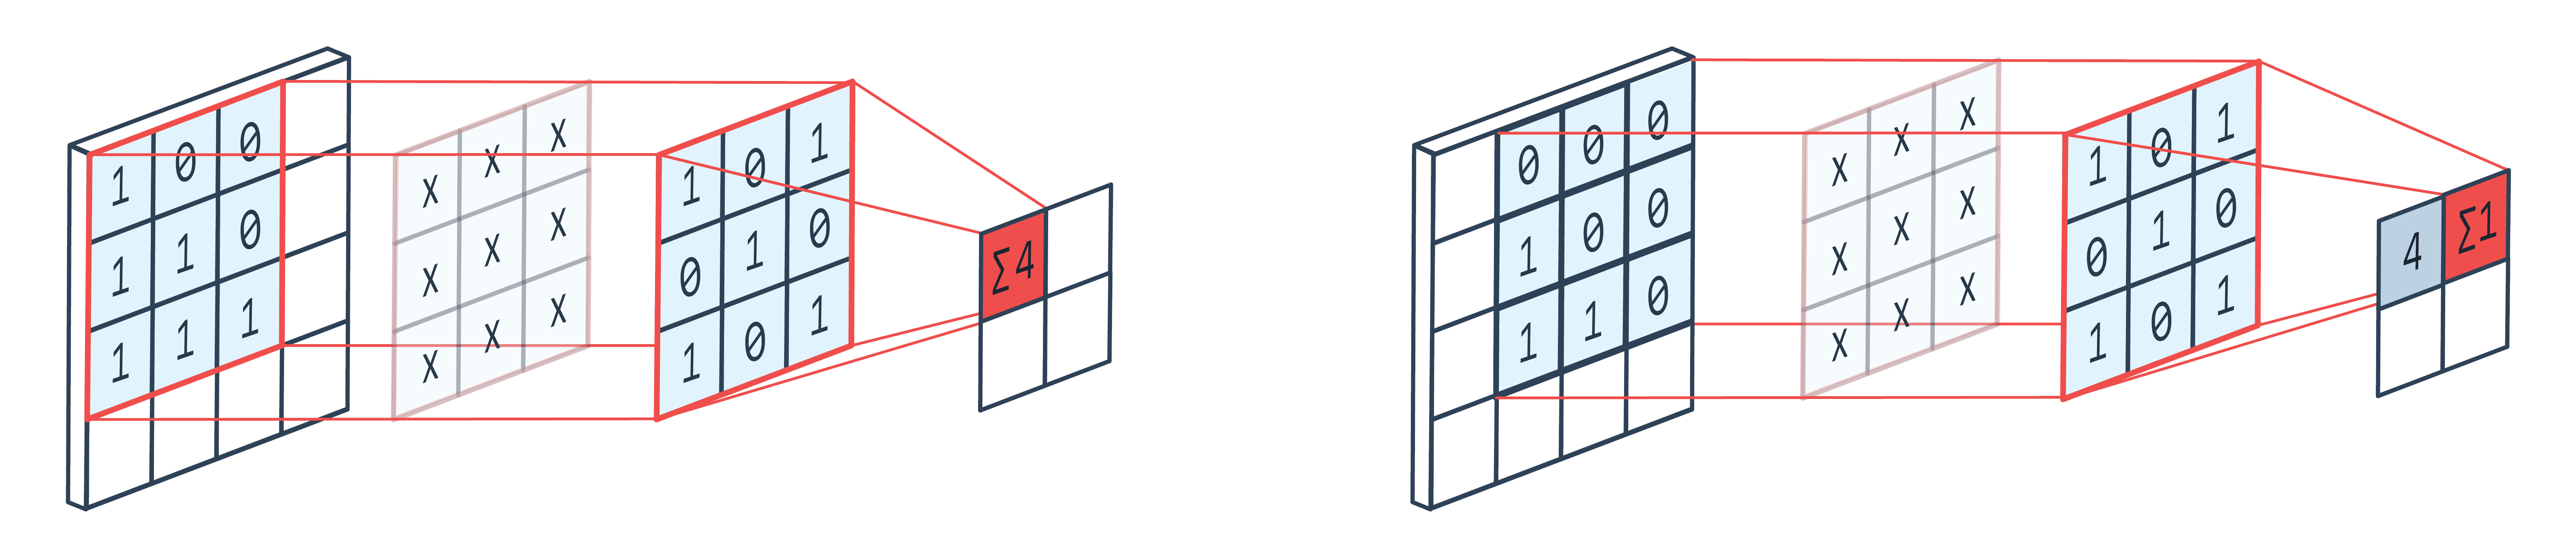
\includegraphics[height=5cm,width=15cm]{Chapitre2/img2.png}
          \caption{Structure de Couche de convolution. \cite{db4}}
          \label{img2}
          \end{figure}
     
     % =========== Pooling Layer ===========
     \subsubsection{Pooling Layer}   
     Ou sous-échantillonnage, Il sert généralement de médiateur entre plusieurs couches de convolution. Max-pooling et Average-pooling sont les stratégies de mise en commun les plus fréquemment utilisées dans les CNN. La mise en commun apporte de nombreux avantages aux CNN. En particulier, la mise en commun vise à empêcher le surajustement en concentrant les données locales avec une fenêtre de mise en commun réduisant ainsi la dimensionnalité des données. La réduction de la dimensionnalité des données permet également de réduire les calculs.
     \begin{figure}[H]
          \centering
          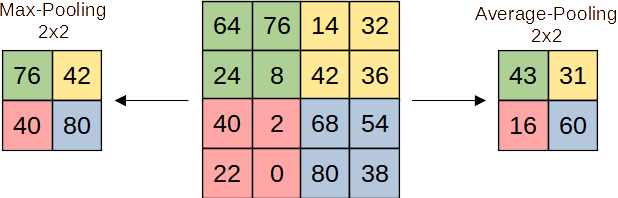
\includegraphics[height=5cm,width=15cm]{Chapitre2/img3.png}
          \caption{Max-pooling et Average-pooling.}
          \label{img3}
          \end{figure}
     
     % =========== Fully Connected Layer ===========
     \subsubsection{Fully Connected Layer (FC)}   
     Cette couche prend la sortie de convolution/polling, l'aplatit et prédit la meilleure étiquette pour décrire l'image. Comme dans un réseau neuronal à anticipation normal, les entrées de la couche entièrement connectée sont multipliées par les poids et additionnées. Ensuite, une fonction d'activation est utilisée pour produire la sortie comme Softmax qui est largement utilisée dans les problèmes de classification.
     \begin{figure}[H]
          \centering
          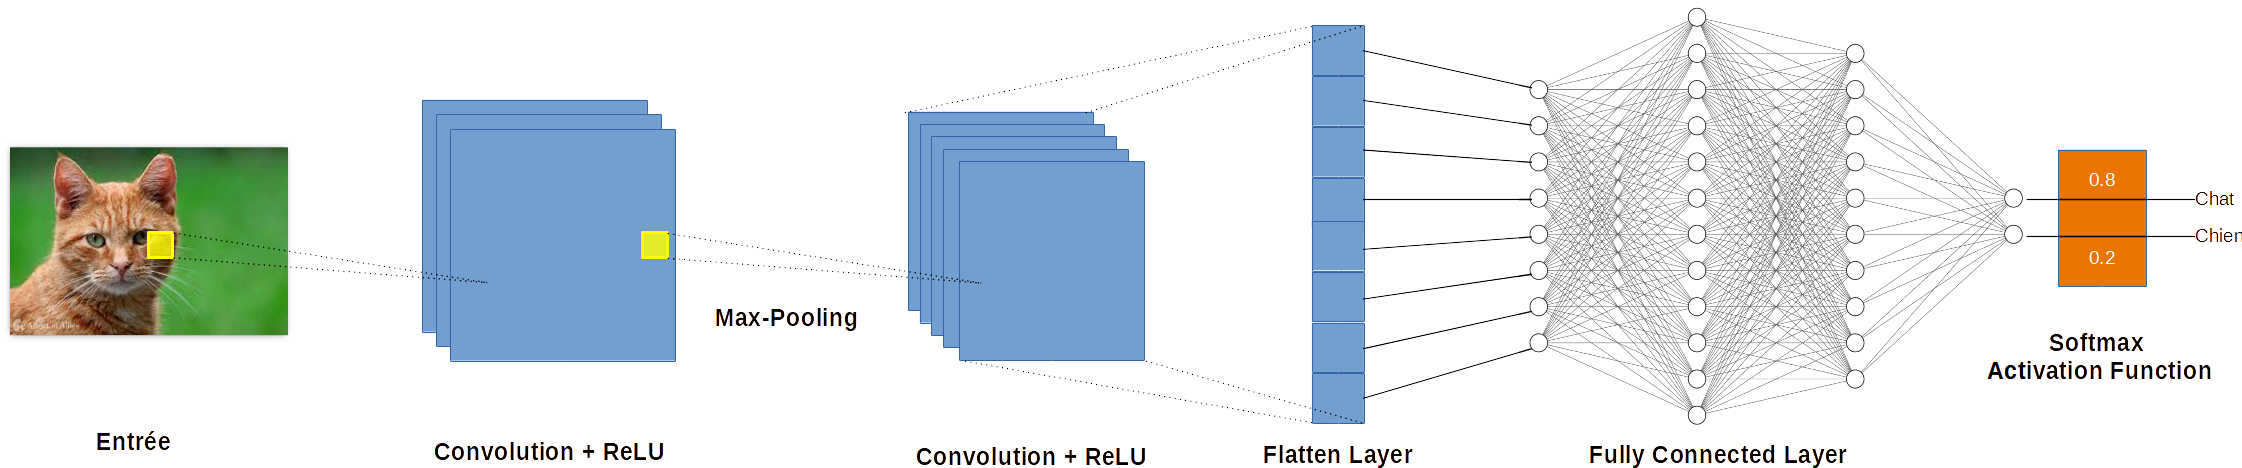
\includegraphics[height=4cm,width=18cm]{Chapitre2/img4.png}
          \caption{Exemple de structure de réseaux de neurones convolutionnels.}
          \label{img4}
          \end{figure}

% =========== Transfer Learning ===========
     \subsection{L'apprentissage par transfert} 
     L'apprentissage par transfert se produit lorsque des modèles existants sont réutilisés pour résoudre un nouveau défi ou problème. L'apprentissage par transfert n'est pas un type distinct d'algorithme d'apprentissage automatique, mais plutôt une technique ou une méthode utilisée lors de la formation de modèles. Les connaissances acquises lors des formations précédentes sont recyclées pour aider à effectuer une nouvelle tâche. La nouvelle tâche sera liée d'une certaine manière à la tâche précédemment formée.

     Le processus prend des parties pertinentes d'un modèle existant et les applique pour résoudre un problème nouveau mais similaire. Un élément clé de l'apprentissage par transfert est la généralisation. Cela signifie que seules les connaissances pouvant être utilisées par un autre modèle dans différents scénarios ou conditions sont transférées. Au lieu que les modèles soient liés de manière rigide à un ensemble de données de formation, les modèles utilisés dans l'apprentissage par transfert seront plus généralisés. Les modèles développés de cette manière peuvent être utilisés dans des conditions changeantes et avec différents ensembles de données.
     \begin{figure}[H]
          \centering
          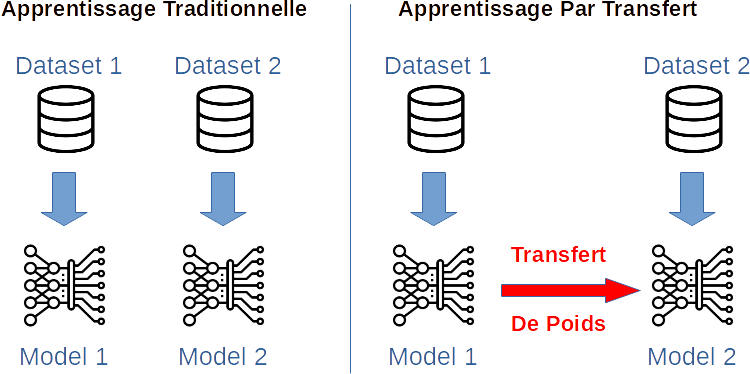
\includegraphics[height=7cm,width=13cm]{Chapitre2/img5.png}
          \caption{Différence entre l'apprentissage traditionnel et l'apprentissage par transfert.}
          \label{img5}
          \end{figure}

% =========== Loss Functions ===========
     \subsection{Fonction de perte pour la détection d'objet}
     En Apprentissage profond, la fonction de perte est aussi appelée fonction de coût. L'objectif principal de la fonction de perte est de mesurer l'écart entre la valeur prédite du réseau et la valeur réelle de l'échantillon. Plus la valeur de la fonction de perte est petite, meilleur est l'apprentissage du modèle de réseau, ce qui prouve la convergence et la robustesse du modèle de réseau. La détection d'objet est divisée en classification d'objet et localisation d'objet. Par conséquent, la fonction de perte inclut la perte de classification et la perte de localisation. La perte de classification appartient à la classification et la perte de localisation appartient à la régression de la boîte englobante.

     % =========== Classification Loss ===========
     \subsubsection{Perte de Classification}
          % =========== Hing Loss ===========
          \paragraph{Hinge loss}
          est une fonction proxy de la fonction de perte $0-1$. Il peut être utilisé comme perte pour le problème de marge maximale dans l'apprentissage automatique ou l'apprentissage en profondeur, et peut être étendu à la perte SVM multi-classes. Plus la valeur après sommation est petite, plus le score de la classe d'erreur sera.
          \begin{center} $L(y)=\sum_{j \neq i}max(0,y_j-y_i+1)$ \end{center}

          Où $y_j$ est le score des autres classes et $y_i$ le score réel declasse.	

          % =========== Cross entropy loss ===========
          \paragraph{Cross entropy loss}
          est également appelée perte de log, qui est utilisée dans le classificateur softmax. La fonction de softmax est de convertir la caractéristique dimensionnelle $(k+1)\times1$ en distribution de probabilité dimensionnelle $(k+1)\times1$. La valeur d'indice de la probabilité maximale est l'étiquette de catégorie de l'échantillon prédit. Par conséquent, selon les caractéristiques de la fonction softmax.
          \begin{center} $L(p,u)=-\sum_{i=0}^{k}u_i log p_i$ \end{center}
          où $p=(p_0,..., p_k)$ est la distribution de probabilité de $K+1$ catégories calculées par le softmax, et u est la véritable étiquette de catégorie. La structure de la fonction montre que la perte d'entropie croisée est la distance entre la valeur prédite et la valeur réelle cible. La structure de la fonction a une optimisation convexe, qui a une bonne convergence lors de la descente du gradient. Il est plus adapté à la classification multi-catégories qu'à Hing loss.
     
     % =========== Localisation Loss ===========
     \subsubsection{Perte de Localistaion}
          % =========== Squared Loss ===========
          \paragraph{Squared Loss}
          est l'une des fonctions de perte de base de la régression de la boîte englobante, également connue sous le nom de perte $L_2$. Il représente la somme des carrés des différences entre la valeur cible et la valeur prédite.
          \begin{center} $L(y, f(x)) = (y - f(x))^2$ \end{center}

          % =========== RSS ===========
          \paragraph{Residual Sum of Squares (RSS)}
          également connue sous le nom de somme des carrés des résidus (SSR) ou somme des carrés de l'estimation des erreurs (SSE), est la somme des carrés des résidus (écarts prédits par rapport aux valeurs empiriques réelles des données). Il s'agit d'une mesure de l'écart entre les données et un modèle d'estimation, tel qu'une régression linéaire.
          \begin{center} $L(Y, F(X)) = \sum_{i=1}^{n}(y_i - f(x_i))^2$ \end{center}

          % =========== MSE ===========
          \paragraph{Mean Squared Error (MSE)}
          mesure la quantité d'erreur dans les modèles statistiques. Il évalue la différence quadratique moyenne entre les valeurs observées et prédites. Lorsqu'un modèle n'a pas d'erreur, le MSE est égal à zéro. À mesure que l'erreur du modèle augmente, sa valeur augmente. L'erreur quadratique moyenne est également appelée écart quadratique moyen (MSD).
          \begin{center} $L(Y, F(X)) = \frac{1}{n}\sum_{i=1}^{n}(y_i - f(x_i))^2$ \end{center}

          % =========== Absolute loss ===========
          \paragraph{Absolute loss}
          est la fonction de perte pour la régression de la boîte englobante, également appelée $L_1$. La différence entre la perte $L_1$ et la perte $L_2$ est que $L_1$ représente la somme des valeurs absolues de la différence entre la valeur cible et la valeur prédite.
          \begin{center} $L(y, f(x))=|y-f(x)|$ \end{center}

          % =========== SAD ===========
          \paragraph{Sum of Absolute Differences (SAD)}
          S'il y a n échantillons avec $L_1$, la fonction de perte prend la forme suivante
          \begin{center} $L(Y, f(X))=\sum_{i=1}^{n}|y_i-f(x_i)|$ \end{center}

          % =========== MAE ===========
          \paragraph{Mean Absolute Error (MAE)}
          La valeur moyenne de SAD est généralement utilisée comme perte de régression, appelée erreur absolue moyenne (MAE)
          \begin{center} $L(Y, f(X))=\frac{1}{n}\sum_{i=1}^{n}|y_i-f(x_i)|$ \end{center}

          La perte $L_1$ et la perte $L_2$ ont leurs propres avantages et inconvénients lorsqu'elles sont utilisées pour la régression de la boîte englobante.
          La perte $L_1$ est plus robuste aux valeurs aberrantes, mais elle a des points où la dérivée ne peut pas être déduite, ce qui rend la descente de gradient inefficace.
          La descente de gradient de la perte $L_2$ est plus précise et simple à calculer, mais plus sensible aux valeurs aberrantes.
          Par conséquent, les avantages de la perte $L_1$ et de la perte $L_2$ sont combinés dans la conception de la fonction de perte de régression de la boîte englobante.

% =========== Backbones =========== 
     \subsection{Architectures CNN populaires} 
     Au fil des ans, de nombreuses architectures de réseaux de neurones convolutionnels ont été introduites, chacune avec sa complexité et sa profondeur uniques en termes de couches en corrélation avec les performances de l'architecture. Les plus notables sont :
     
          % =========== AlexNet =========== 
          \subsubsection{AlexNet} \cite{alex_paper}
          Alex Krizhevsky en collaboration avec Ilya Sutskever et Geoffrey Hinton. en 2012, a développé un réseau de neurones convolutifs composé de 8 couches, dont 5 sont convolutives et 3 sont entièrement connectées. Le réseau s'appelle AlexNet. il a amélioré LeNet-5 en ajoutant plus de couches et en contenant environ 60 millions de paramètres. Les unités linéaires rectifiées (ReLU) sont utilisées pour la première fois comme activations dans AlexNet au lieu des activations sigmoïdes et tanh pour ajouter de la non-linéarité.
          \begin{figure}[H]
               \centering
               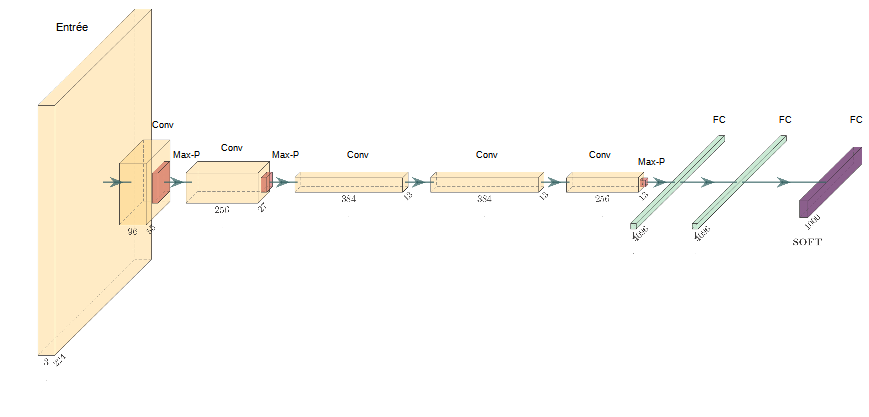
\includegraphics[height=9cm,width=15cm]{Chapitre2/img6.png}
               \caption{Architecture de AlexNet.}
               \label{img6}
               \end{figure}

          % =========== VGG-16 ===========
          \subsubsection{VGG-16} \cite{vgg_paper}
          est l'une des architectures les plus utilisées dans la détection d'objets et a 	réalisé des performances intéressantes, elle est sortie en 2014, composée de 13 couches convolutives et 3 entièrement connectées avec activation ReLU. VGG-16 fournit plus de couches par rapport à AlexNet et utilise des filtres plus petits de 2x2 et 3x3. Il comprend 138 millions de paramètres.
          \begin{figure}[H]
               \centering
               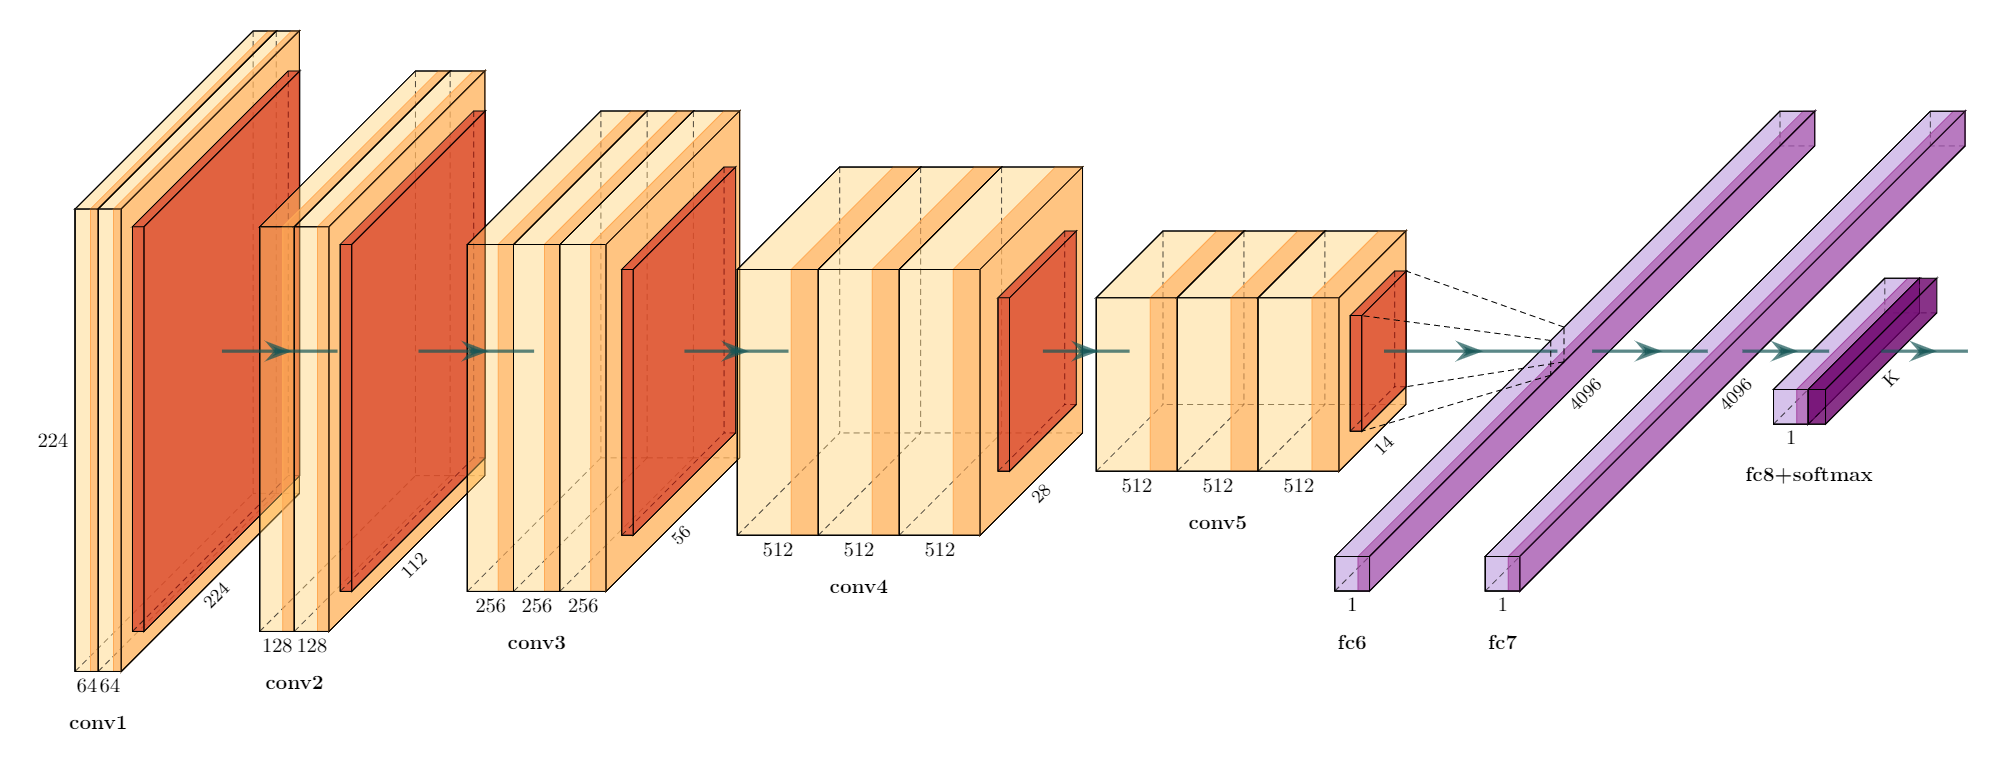
\includegraphics[height=9cm,width=15cm]{Chapitre2/img7.png}
               \caption{Architecture de VGG-16.}
               \label{img7}
               \end{figure}

          % =========== ResNet ===========
          \subsubsection{ResNet} \cite{res_paper}
          Les réseaux de neurones convolutifs sont devenus de plus en plus profonds avec l'ajout de couches, mais une fois la précision saturée, elle chute rapidement, ce phénomène appelé dégradation. Pour résoudre ce problème, He et al. en 2015 ont développé des ResNets basés sur les résidus. Les résidus sont essentiellement des connexions de raccourci, une pile de couches définies de telle sorte que la sortie d'une couche est prise et ajoutée à une autre couche plus profonde dans le réseau. Étant donné que le module d'apprentissage résiduel résout le problème de la dégradation de la formation, la profondeur du réseau est augmenté et les performances sont continuellement améliorées.

          Il existe de nombreuses variantes de ResNets, par exemple, ResNet-50 qui est composé de 26 millions de paramètres, ResNet-101 avec 44 millions de paramètres et ResNet-152 qui est plus profond avec 152 couches, les deux sont largement utilisés dans la détection d'objets.
          \begin{figure}[H]
               \centering
               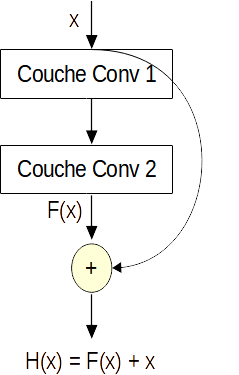
\includegraphics[height=8cm,width=5cm]{Chapitre2/img8.png}
               \caption{Structure d'un bloc résiduel.}
               \label{img8}
               \end{figure}
          
          % =========== GoogLeNet ===========
          \subsubsection{GoogLeNet} \cite{googlenet_paper}
          Aussi appelé Inception V1, GoogLeNet est un petit réseau développé par Szegedy et al. en 2014. Leur méthode est différente de celle de VGGNet et AlexNet. Ils ont proposé une nouvelle notion connue sous le nom Inception Block, où elle intègre des transformations convolutives à plusieurs échelles. Inception Block comprend des filtres de différentes tailles 1x1, 3x3 et 5x5. Il utilise une convolution 1x1 au milieu du réseau pour réduire la dimensionnalité et ils ont choisi d'utiliser Max-Pooling au lieu de couches entièrement connectées. Le réseau est composé de 22 couches avec 5 millions de paramètres. GoogLeNet est principalement utilisé dans le modèle de détection d'objets YOLO.
          \begin{figure}[H]
               \centering
               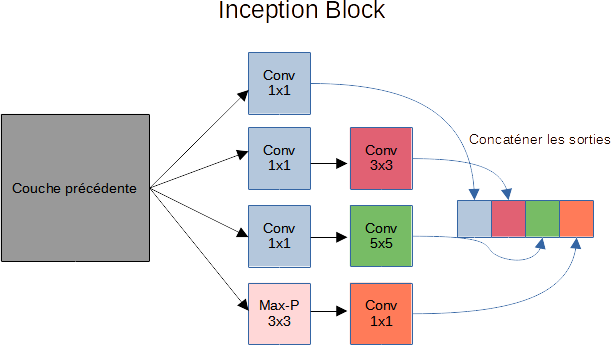
\includegraphics[height=8cm,width=12cm]{Chapitre2/img9.png}
               \caption{Structure de Inception Block.}
               \label{img9}
               \end{figure}

           % =========== Darknet-53 ===========
           \subsubsection{Darknet-53} \cite{darknet_paper}
           Il a été introduit en 2018 par Joseph Redmon Ali Farhadi, il sert d'architecture de YOLOv3. c'était une amélioration de son prédécesseur Darknet-19 qui était l'architecture de YOLOv2. il se compose de 53 couches convolutionnelles qui servent de base au réseau de détection d'objets ou à un extracteur de caractéristiques. inclure l'utilisation de connexions résiduelles. Après chaque couche convolutive, un groupe résiduel a différents blocs résiduels tels que 1x, 2x, 4x et 8x. Pour sous-échantillonner la dimension spatiale des cartes d'entités, une convolution striée avec une foulée de 2 est utilisée avant chaque groupe résiduel. Cela a permis d'éviter la perte de fonctionnalités de bas niveau et d'encoder des informations de position utiles pour la détection d'objets.
           \begin{figure}[H]
                \centering
                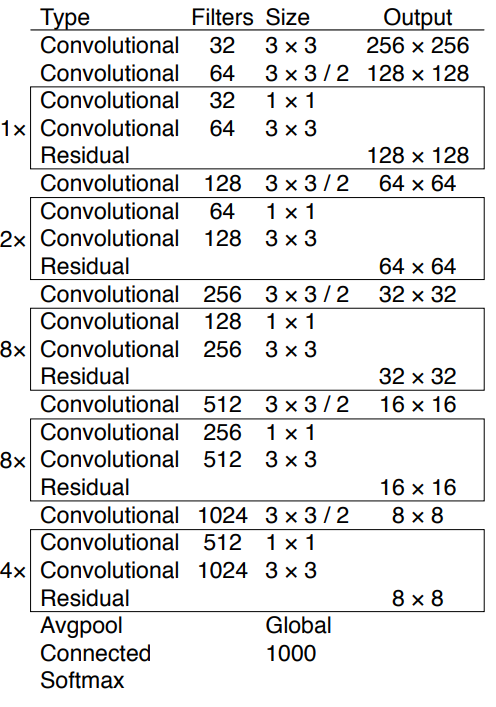
\includegraphics[height=8cm,width=7cm]{Chapitre2/img10.png}
                \caption{Architecture de Darknet-53.}
                \label{img10}
                \end{figure}


\section{Les méthodes de détections d'objets basées sur l'apprentissage profond} 
Les méthodes actuelles de détection d'objets sont divisées en 2 catégories :
% =========== Two-Stage ===========
     \subsection{Détecteurs à Deux-étapes}
     Ce type de détecteurs sépare la tâche de localisation d'objets de la tâche de classification d'objets. Il génère d'abord la proposition de région, puis classe la région. Le principal avantage est la haute précision de détection et le principal inconvénient est la lenteur vitesse de détection.
     
     % =========== RCNN ===========
     \subsubsection{RCNN} \cite{rcnn_paper}
     Il a été introduit par Ross Girshick et al en 2004. Il extrait d'abord 2000 régions de l'image et on les appelle des propositions de région en utilisant un algorithme de recherche sélective. Ces 2000 propositions de régions candidates sont déformées en un carré et introduites dans un réseau neuronal convolutionnel qui produit un vecteur de caractéristiques de 4096 dimensions en sortie. Le CNN agit comme un extracteur de caractéristiques et la couche dense de sortie se compose des caractéristiques extraites de l'image et les caractéristiques extraites sont introduites dans un SVM pour classer la présence de l'objet dans cette proposition de région candidate. La régression de la boîte englobante et la suppression non maximale (NMS) seront effectuées pour effectuer un réglage fin de la boîte englobante.
     \begin{figure}[H]
          \centering
          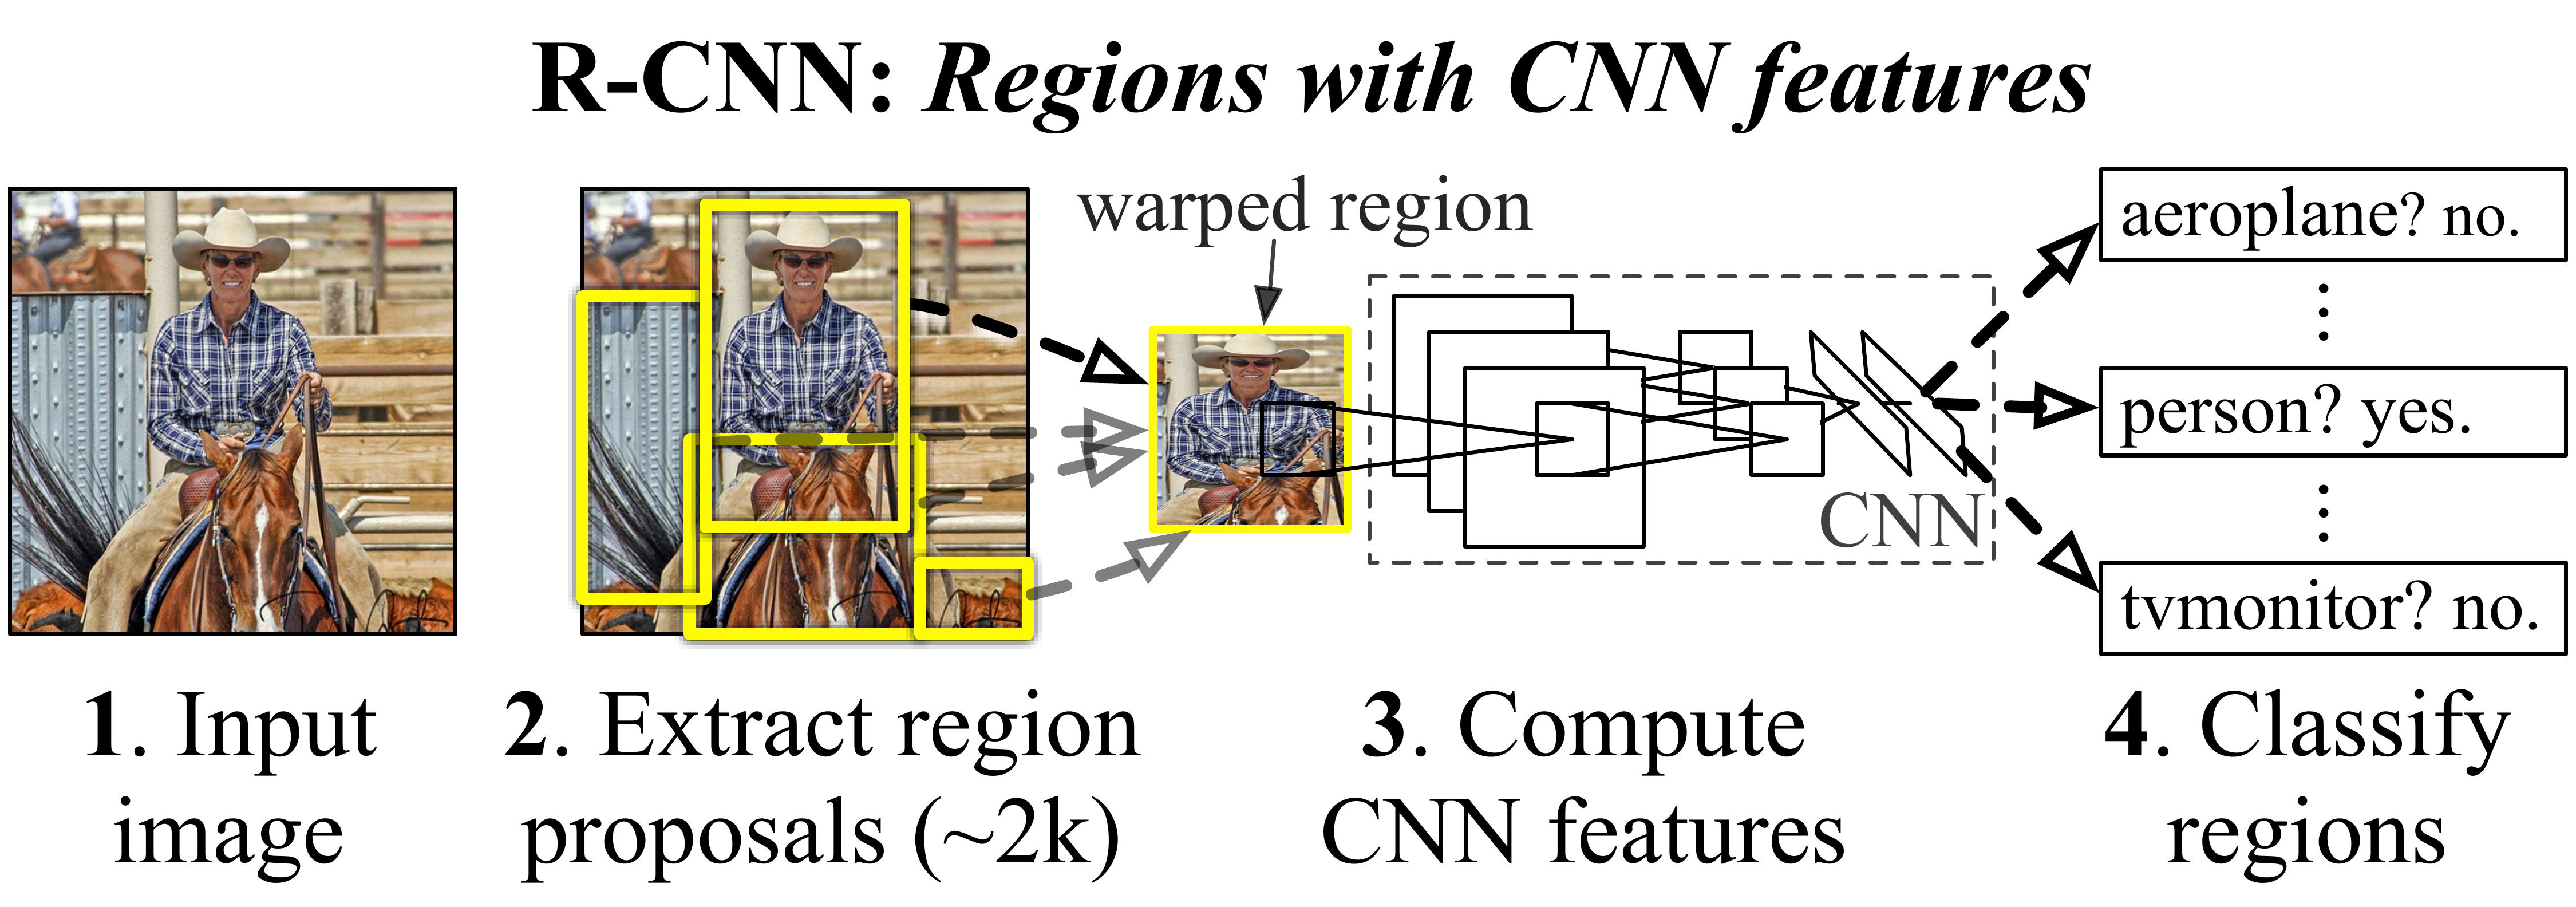
\includegraphics[height=5cm,width=15cm]{Chapitre2/img11.jpg}
          \caption{Architecture de RCNN}
          \label{img11}
          \end{figure}
     \begin{figure}[H]
          \centering
          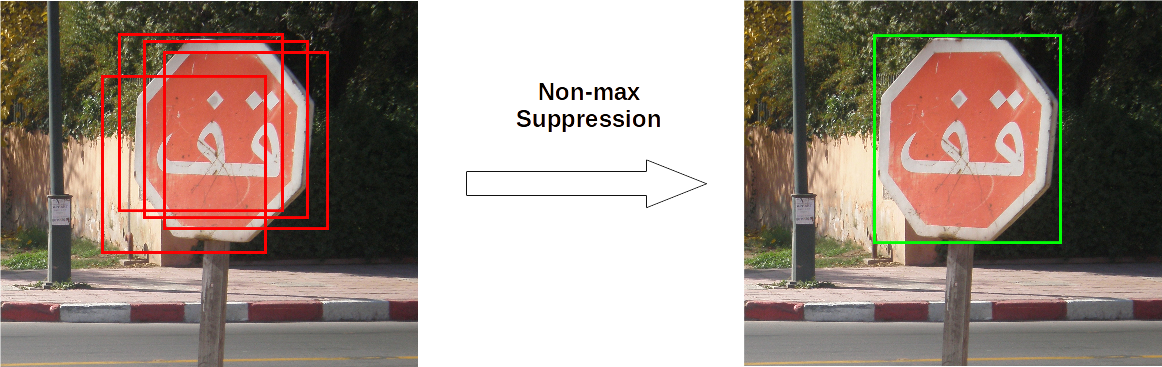
\includegraphics[height=5cm,width=15cm]{Chapitre2/img12.png}
          \caption{Suppression non maximale (NMS).}
          \label{img12}
          \end{figure}

     % =========== Fast-RCNN ===========
     \subsubsection{Fast-RCNN} \cite{fast_rcnn_paper}
     R.Girshick et al. a proposé couche de pooling de région d'intérêt (Region of Interst, ROI),il mappe différentes régions de caractéristiques sur des vecteurs de caractéristiques de taille fixe et les envoie à la couche entièrement connectée (FC). puis le softmax prédit les catégories d'objets et la régression de la boîte englobante localise avec précision l'emplacement de l'objet. Un autre changement est qu'il utilise la perte multi-tâches conjointement pour former la classification et la régression de la boîte englobante, ce qui augmente considérablement la vitesse.
     \begin{figure}[H]
          \centering
          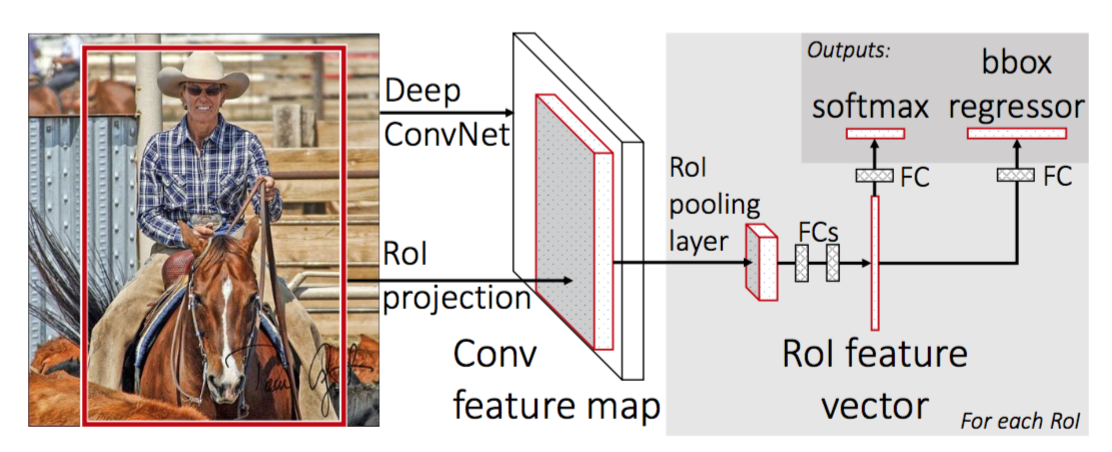
\includegraphics[height=5cm,width=15cm]{Chapitre2/img13.png}
          \caption{Architecture de Fast-RCNN}
          \label{img13}
          \end{figure}

     % =========== Faster-RCNN ===========
     \subsubsection{Faster-RCNN} \cite{faster_rcnn_paper}
     RCNN et Fast-RCNN avaient un goulot d'étranglement qui est l'algorithme de recherche sélective qui est utilisé dans la phase de proposition de région. il doit rechercher toutes les propositions de région dans l'image et les mapper dans les cartes d'entités, ce qui prend beaucoup de temps. Par conséquent, Shaoqing Ren et al ont proposé un réseau de proposition régional (RPN), il s'est intégré dans le réseau qui partage les caractéristiques de convolution de l'image complète avec le réseau de détection qui a permis au RPN d'être implémenté dans le GPU, ce qui a donné un coût quasi nul de exécution. RPN prend en entrée la carte de caractéristiques de convolution générée par la couche dorsale et génère les ancres générées par la convolution de fenêtre coulissante appliquée sur la carte de caractéristiques d'entrée.
     \begin{figure}[H]
          \centering
          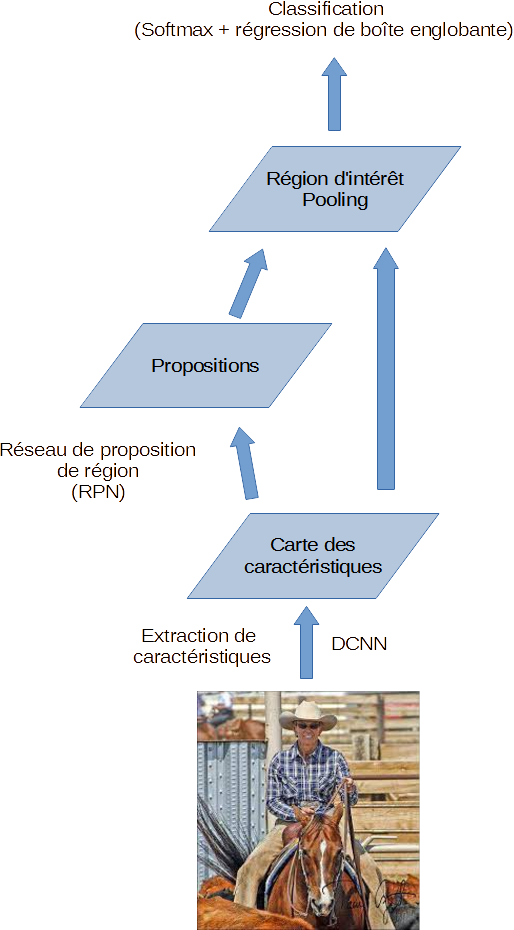
\includegraphics[height=14cm,width=7cm]{Chapitre2/img14.png}
          \caption{Architecture de Faster-RCNN}
          \label{img14}
          \end{figure}

% =========== One-Stage ===========
     \subsection{Détecteurs à Un-étapes}
     Contrairement aux détecteurs à deux étapes, ces modèles ignorent l'étape de proposition de région des modèles à deux étages et exécutent la détection directement sur un échantillonnage dense d'emplacements. Ils considèrent généralement toutes les positions sur l'image comme des objets potentiels et essaient de classer chaque région d'intérêt comme arrière-plan ou comme objet cible.

     % =========== YOLO ===========
     \subsubsection{YOLO (You Only Look Once)} \cite{yolo_paper}
     a été publié pour la première fois par Joseph Redmon et al. en 2015, le réseau utilisé utilise un GoogLeNet modifié comme réseau backbone. il se compose de 24 couches convolutionnelles et de 2 couches entièrement connectées avec une entrée réseau de 448 × 448 images. Il divise l'image complète en grilles S×S. Chaque cellule de grille est responsable de la détection du centre de l'objet tombant dans la cellule de grille. Chaque cellule de la grille prédit les probabilités de classe C, les boîtes englobantes B et les scores de confiance, et l'image complète est codée pour produire le tenseur SxSx(5B+C).
     \begin{figure}[H]
          \centering
          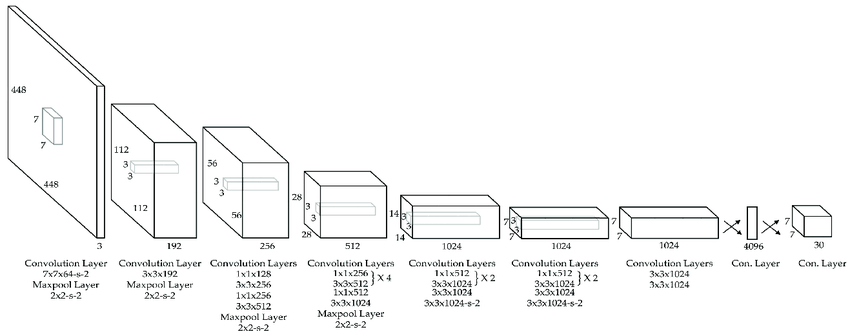
\includegraphics[height=7cm,width=14cm]{Chapitre2/img15.png}
          \caption{Architecture de YOLO (You Only Look Once)}
          \label{img15}
          \end{figure}

     % =========== YOLOv3 ===========
     \subsubsection{YOLOv3} \cite{yolov3_paper}
     été introduit par Redmon J et Farhadi A 2018, il est basé sur l'architecture Darknet-53 qui combine des blocs résiduels et FPN (Feature Pyramid Network) est un extracteur de caractéristiques qui prend une image à échelle unique d'une taille arbitraire en entrée et des sorties proportionnellement dimensionnées cartes de fonctionnalités à plusieurs niveaux, ce qui donne de bonnes performances sur une large gamme de résolutions d'entrée.
     \begin{figure}[H]
          \centering
          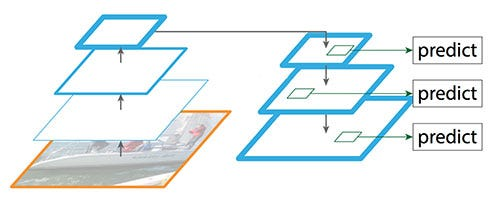
\includegraphics[height=5cm,width=9cm]{Chapitre2/img16_.jpg}
          \caption{Feature Network Pyramid (FNP)}
          \label{img16_}
          \end{figure}
     \begin{figure}[H]
          \centering
          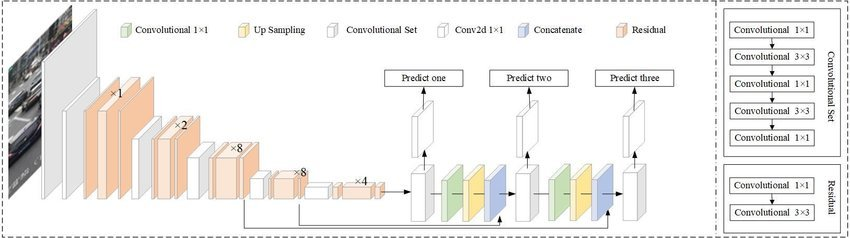
\includegraphics[height=6cm,width=14cm]{Chapitre2/img16.jpg}
          \caption{Architecture de YOLOv3}
          \label{img16}
          \end{figure}
     
          
     % =========== SSD ===========
     \subsubsection{SSD (Single Shot MultiBox Detector)} \cite{ssd_paper}
     il a été publié par C. Szegedy et al en 2016. il a utilisé VEGG16 comme réseau principal pour l'extraction de caractéristiques tout en remplaçant les couches entièrement connectées par des couches convolutives et en ajoutant 4 autres couches convolutives. Le réseau est divisé en 6 étapes. Chaque étape extrait des cartes de caractéristiques de différents niveaux sémantiques et effectue une classification d'objets et une régression par boîte englobante.
     \begin{figure}[H]
          \centering
          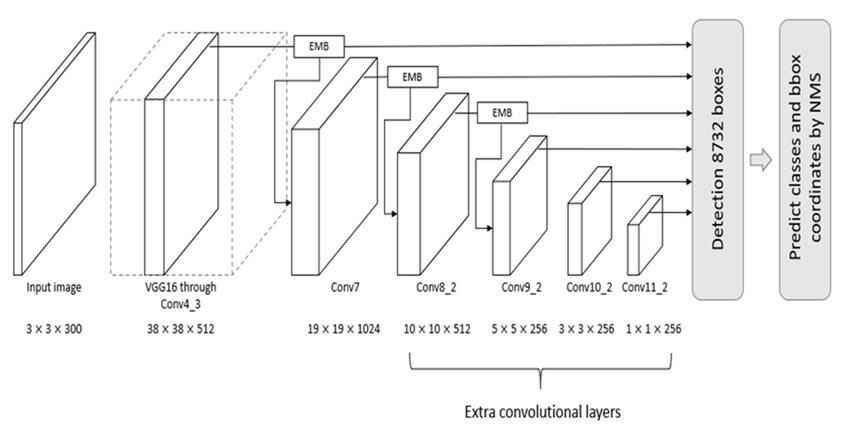
\includegraphics[height=7cm,width=14cm]{Chapitre2/img17.png}
          \caption{Architecture de SSD (Single Shot MultiBox Detector)}
          \label{img17}
          \end{figure}

\section{Métriques pour l'évaluation des systèmes de détection d'objets} 

\section{Bases de données d'évaluation} 
Les bases de données d'évaluation jouent un rôle très crucial dans la recherche, ceux sont l'un des facteurs les plus importants pour les progrès dans le domaine, malheureusement les données sont plus difficiles et plus coûteuses à générer. Au cours de la dernière décennie, un certain nombre d'ensembles de données ont été rendus publics pour évaluer les algorithmes de détection d'objets. Ces ensembles de données sont collectés à partir de différents scénarios et peuvent donc être utilisés comme référence pour les applications. Ci-dessous, nous décrivons les ensembles de données  les plus populaires utilisés pour l'évaluation dans ce domaine:

\begin{itemize}
\item Microsoft COCO \cite{db1}

\item ImageNet \cite{db2}
\item 
\item 
\item 
\end{itemize}



\section{Conclusion} 
